\begin{problem}{데굴데굴}{standard input}{standard output}

종훈이는 질 좋은 문제와 푸짐한 상품이 주어지는 서울대학교 프로그래밍 경시대회에 출전했다. 하지만 참가 신청을 할 때 실수를 하는 바람에 숨겨진 난이도인 Div. 0 난이도에 신청하고 말았고, $N = 1,000$짜리 Travelling salesman problem을 풀면서 고통받고 있었다. 결국, 그 문제를 NP(Not my Problem)-hard 문제로 결론지은 종훈이는 대회장에 가지고 온 물병을 가지고 놀면서 남은 시간을 보내기로 했다.

종훈이가 가지고 온 물병은 밑면이 볼록다각형인 직각기둥 모양이고, 물이 조금 들어 있다. 종훈이는 물병을 완전히, 즉 두 밑면에 속하지 않은 변이 모두 밑면과 평행하도록 눕혀 놓고 데굴데굴 굴려 보았다. 그리고 물병이 구르면서 물병의 밑면에서 물이 차지하는 영역이 다양한 모양으로 바뀌는 걸 지켜보다가, 문득 이 영역을 자기가 원하는 개수만큼의 변을 가진 다각형으로 만들 수 있는지 궁금해졌다. 종훈이는 자신이 이 문제를 풀 수 있을 거라 생각했지만, 이미 너무 지쳐 있었기 때문에 대신 Div. 1 대회장에서 열심히 문제를 풀고 있는 당신에게 도움을 요청했다.

종훈이는 수시로 물을 마시거나 정수기에서 다시 물을 떠 오고, 그 때마다 당신에게 도움을 요청할 것이다. 편의를 위해 물병의 높이는 $1cm$이며, 물병의 물은 물병을 기울이는 즉시 평형을 되찾는다고 가정한다.

\InputFile
첫 번째 줄에 물병의 밑면을 이루는 꼭짓점의 수 $N$($3 \le N \le 500,000$), 종훈이가 도움을 요청한 횟수 $M$($1 \le M \le 50$)이 주어진다.

두 번째 줄부터 $N$개의 줄에 걸쳐 물병의 밑면을 이루는 꼭짓점의 $x$ 좌표와 $y$ 좌표가 공백으로 구분되어 주어진다. 이는 물병의 밑면을 $1cm$ 단위로 격자가 그려진 좌표평면에 본뜬 뒤 임의의 꼭짓점에서 시작하여 반시계방향으로 돌면서 만나는 꼭짓점들의 좌표를 순서대로 기록한 값이다. 각 좌푯값은 모두 정수이며 $-100,000,000$ 이상 $100,000,000$ 이하이다. 세 꼭짓점이 한 직선 위에 있는 경우는 없다.

$N + 2$번째 줄부터 $M$개의 줄에 걸쳐 각각의 요청에 대해 물병에 들어 있는 물의 양을 의미하는 정수 $W$($1 \le W \le$ 물병의 부피, 단위는 $cm^{3}$)가 주어진다.

\OutputFile
$M$개의 줄에 걸쳐 $m$번째 줄에 $m$번째 요청에 대해 물병을 눕혀 놓고 굴렸을 때 물병의 밑면에서 물이 차지하는 영역이 가질 수 있는 가장 적은 변의 수와 가장 많은 변의 수를 공백으로 구분하여 출력한다.

\Example

\begin{example}
\exmp{5 2
-5 2
1 -1
4 -1
4 5
1 5
18
24}{3 5
4 6}%
\end{example}

\Notes
\begin{center}
  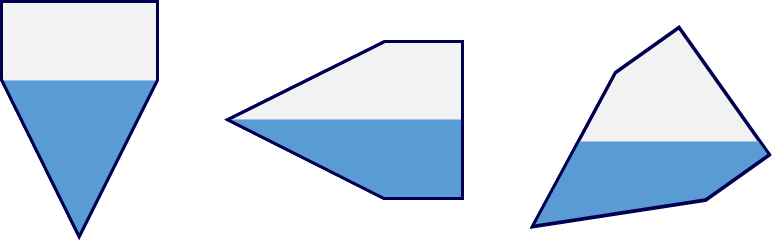
\includegraphics[width=0.5\textwidth]{roll.png}
\end{center}

위의 그림은 첫 번째 요청에 대해 물이 차지하는 영역이 삼각형, 사각형, 오각형을 이루는 경우이다.

\end{problem}
